
\documentclass[11pt
  , a4paper
  , article
  , oneside
%  , twoside
%  , draft
]{memoir}

\usepackage{control}
\usepackage[numbers]{natbib}

\begin{document}
\newcommand{\technumber}{
  RAON Control-Document Series\\
  Revision : v0.1.4,   Release : Oct, 19, 2014}
\title{\textbf{Naming Convention \\ for the RAON Control System}}

\author{Jeong Han Lee\thanks{jhlee@ibs.re.kr} \\
  Control Team \\
  Rare Isotope Science Project\\
  Institute for Basic Science\\
  Daejeon, South Korea
}
\date{\today}

\renewcommand{\maketitlehooka}{\begin{flushright}\textsf{\technumber}\end{flushright}}
%\renewcommand{\maketitlehookb}{\centering\textsf{\subtitle}}
%\renewcommand{\maketitlehookc}{C}
%\renewcommand{\maketitlehookd}{D}

\maketitle

\begin{abstract}
A naming convention for the RAON control system is a convention for naming signals and devices which will be used for the RAON accelerator in order to control the whole accelerator and monitor its signals as well. This document shows how to use the naming convention in any sub-system so that we may eliminate a typical burden to integrate them all into the RAON accelerator control system framework. 
\end{abstract}



\chapter{Motivation}
The naming convention is a rule for matching signals, which are from devices and equipment of an accelerator, to signals. And an efficient naming rule quickly and easily lets us to know what the signal is, where the signal comes from, and which device or equipment is related with the signal. Therefore, an accelerator facility needs a well-defined naming convention.  

To avoid confusion and conflicts, names of all devices, equipment and control system signals must be unique. In the case of a control system, signals uniqueness is a strict requirement. In EPICS based control system, signals are represented with process variables (PV). A PV is a named piece of data that is transmitted over the network and to ensure error free communication between different subsystems each PV name must be unique. 

Another benefit of the naming convention is that names created according to a naming convention can provide some information about the device, equipment or signal. For a control system, signal that includes the name of the associated device, the location of the device within the logical structure of the facility, and the function or parameter the PV is associated with. It is recommended that the naming convention is such that names, when written, are difficult to confuse with other names. For example, names that differ only in case, the use of characters \texttt{l} (lower-case L), \texttt{I} (upper-case I) and \texttt{1} (one), letters \texttt{V} and \texttt{W}, etc., should be avoided.


\chapter{Scope of the Naming Convention \cite{DaveGurd,NCSNS,NCESS}}
The naming convention should apply to all devices (beam instrumentation, sensors, actuators, etc.), equipment (power supplies, magnets, cavities, targets, moderators, instruments, etc.) and signals in technical systems and conventional facilities. And these requirements do not apply to cable numbering, pipe numbering, or location designations throughout facility. 

The names determined through this naming convention should be used on operator screens, in the inventory system, drawings, design schematics, computer software, project databases, equipment name tags, test procedures, and other sources of technical information at RAON.


\chapter{Naming Convention Scheme}
Since the RAON integrated control system uses the EPICS framework, a standard EPICS naming convention is the basis of the naming convention for the RAON control system. The format is shown as 
\begin{equation*}
\underbrace{\mathbf{SYS-SUBSYS}}_\text{a system element}\mathbf{:}\overbrace{\mathrm{DEVXXX(-SUBDEVXXX)}}^\text{a device element}\mathbf{:}\underbrace{SignalName\mathbf{.}\mathrm{Field}}_\text{a signal element}
\end{equation*} 
, where 

\begin{itemize}
\item \textbf{SYS}    : a system name which is \texttt{UPPERCASE} or \texttt{UpperCamelCase}. 
\item \textbf{SUBSYS} : a sub-system name which is \texttt{UPPERCASE} or \texttt{UpperCamelCase}. 
\item \textbf{DEV} : a device name which is \texttt{UPPERCASE} or \texttt{UpperCamelCase}.
\item \textbf{SUBDEV} : a sub-device which is \texttt{UPPERCASE} or \texttt{UpperCamelCase}, and is an empty option for future expansion.
\item \textbf{XXX}  : a device numbering assigned by a system or a sub-system. Numbering sequences starting at \textbf{1} in the RAON Naming convention. So the first device will be \textbf{001}. We do not use the Zero-based numbering \cite{ZERONUM}. 
\item \textbf{SignalName} : a signal name which is \texttt{UPPERCASE} or \texttt{UpperCamelCase}. Also it has two parts as Quantities and Attributes.
\item \textbf{Field} : a field name which is \texttt{UPPERCASE} and for the EPICS internal usage.
\end{itemize}

 
\chapter{Naming Syntax Rules}

When applying the naming convention to any subsystem signals, one should follow the following syntax rules :
\begin{enumerate}
\item  Allowed characters for names are alphanumeric characters (\texttt{A-Z}, \texttt{a-z}, and \texttt{0-9}) and two separator characters (\texttt{-}, \texttt{:})
  \begin{itemize}
    \item Avoid using the uppercase letter \texttt{O}, be confused with the number \texttt{0}.
    \item Avoid using the uppercase letter \texttt{I}, be confused with the number \texttt{1}.
  \end{itemize}
\item The delimiter \texttt{:} separates name elements. There are three name elements as follows: the system, device, and signal name element. 
\item The delimiter \texttt{-} separates system/sub-system segments and device/sub-device segments.

\item All three name elements are obligatory for signals. Device names may omit the signal name element when reference is made only to the device. Conventional facility names may omit device and signal name elements when reference is only being made to the system level (building) name and not to items or devices within the building.

\item If additional segmentation of the system or subsystem is required or for better clarity, an number can be appended to the system or subsystem segments, which we can call as \textit{system or subsystem numbering}.

\item Letter case are used to improve readability but are not used to distinguish between names. That is, there will not be two names for which the only difference is the letter case.

\item The first letter of a word or abbreviation is uppercase and succeeding letters are lowercase. Acronyms are all uppercase.

\item The device numbering can be omitted if there is only one instance of the device present in the system/subsystem combination. For example, the event generator \texttt{Evg} instead of \texttt{Evg001} if there is only one event generator in the timing system. The device numbering can also be descriptive if the scope of the device allows it.

\item Vendor specific, contemporary, or \textit{funny} naming should be avoided. 

%\item Configuration PVs which reflect actual value which was applied should be marked by the RBV suffix.

\end{enumerate}

\chapter{System element}

\section{System code : \texttt{SYS}}
A system is at the highest level in the logical structure of the RAON accelerator. Table \ref{table:systemcodes} shows an incomplete list of the system codes. In case of multiple systems sharing the same system code it
is possible to differentiate between them by adding a number (\textit{a system numbering}). Figure \ref{fig:naming-layout} shows the system code according to the site layout. 


\begin{center}
\begin{longtable}[t]{>{\raggedleft\arraybackslash}p{3cm} |p{7cm}| p{3cm}}
\caption{System Codes}
\label{table:systemcodes}\\
\toprule
\texttt{System} & \textbf{code description} &  \textbf{Sectors}\\
\midrule
\endfirsthead
%%\multicolumn{4}{c}%
%%{\tablename\ \thetable\ -- \textit{Continued from previous page}} \\
\toprule
\texttt{System} & \textbf{code description} &  \textbf{Sectors}\\
\midrule
\endhead
\midrule \multicolumn{3}{r}{\tablename\ \thetable\ -- \textit{Continued on next page}} \\
\bottomrule
\endfoot
\bottomrule
\endlastfoot
&\\
\texttt{ECR11}  & 1st ECR-IS for SCL1 & Injector\\
\texttt{ECR12}  & 2nd ECR-IS for SCL1 & Injector \\
\texttt{LEBT11} & 1st section of LEBT for SCL1& Injector\\
\texttt{LEBT12} & 2nd section of LEBT for SCL1& Injector\\
\texttt{RFQ1}   & RFQ for SCL1 & Injector\\
\texttt{MEBT1}  & MEBT for SCL1 & Injector\\
\texttt{ECR31}  & ECR-IS for SCL3 & Injector\\
\texttt{LEBT31} & 1st section of LEBT for SCL3 & Injector\\
\texttt{LEBT32} & 2nd section of LEBT for SCL3 & Injector\\
\texttt{RFQ3}   & RFQ for SCL3 & Injector\\
\texttt{MEBT3}  & MEBT for SCL3 & Injector\\
&\\
\texttt{SCL11} & 1st section of SCL1 & SCL\\
\texttt{SCL12} & 2nd section of SCL1 & SCL \\
\texttt{SCL21} & 1st section of SCL2 & SCL\\
\texttt{SCL22} & 2nd section of SCL2 & SCL \\
\texttt{SCL31} & 1st section of SCL3 & SCL\\
\texttt{SCL32} & 2nd section of SCL3 & SCL \\
&\\
\texttt{IF}    & IF System  & IF \\
\texttt{Cyc}   & Cyclotron  & Cyclotron \\
\texttt{Cryo}  & Cryogenic System & Cryogenic\\
\texttt{Ctrl}  & Control System   & Control \\
&\\
\texttt{Elec}  & Power and Communication & Conventional\\
\texttt{Mech}  & HVAC and utilities system & Conventional \\
\texttt{Dmp}   & Dump & TBD \\
\texttt{FA}    & Fire Alarm & Safety\\
\texttt{CF}    & Conventional Facility & Conventional\\
\texttt{FE}    & Front End & TBD \\
&\\
\end{longtable}
\end{center}


\begin{figure}[!htb]
  \centering
  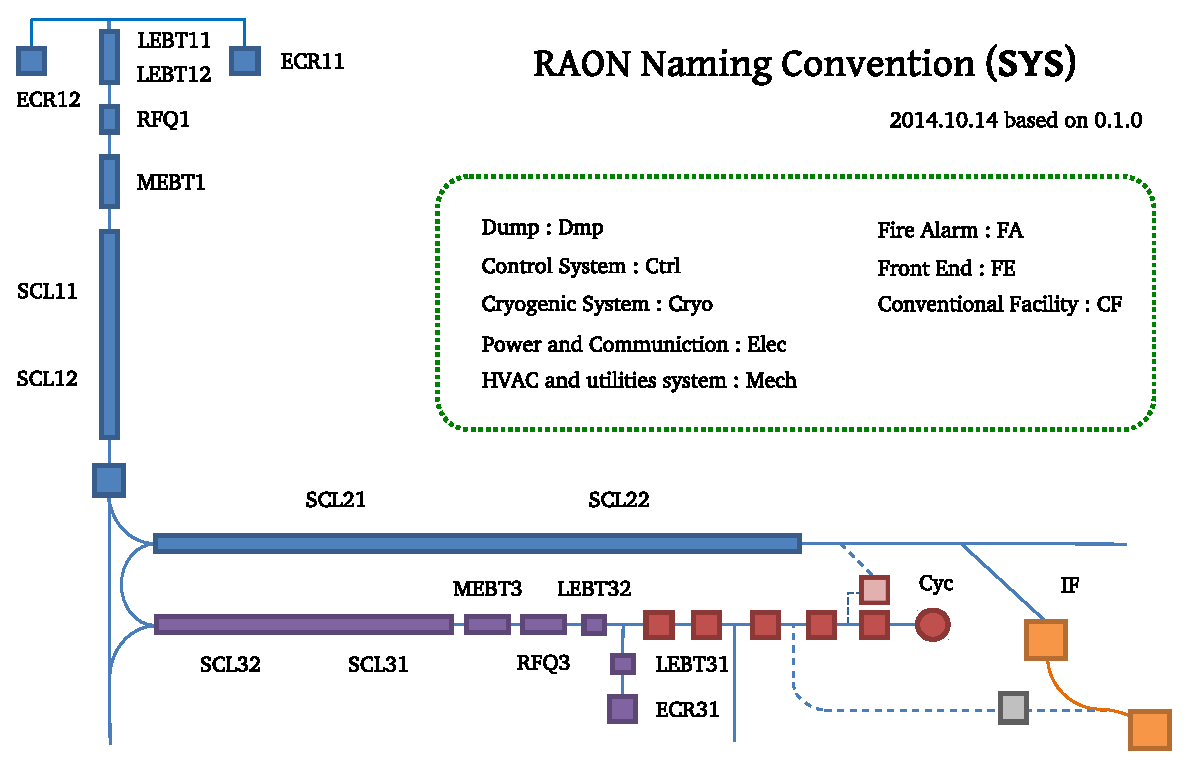
\includegraphics[width=0.98\textwidth]{./images/naming-layout.eps}
  \caption{
            System Code \textbf{SYS} according to the RAON Site layout in the RAON control system naming convention.
          }
  \label{fig:naming-layout}   
\end{figure}



\section{Subsystem code : \texttt{SUBSYS}}
A subsystem is at the second highest level in the logical structure of the RAON accelerator system. It is a grouping of devices that fulfill a specific function. Table \ref{table:subsystemcodes} shows an incomplete list of the subsystem codes. In case of multiple subsystems sharing the same subsystem code, it is possible to differentiate between them by adding a number (\textit{a subsystem numbering}).


\begin{center}
\begin{longtable}[t]{>{\raggedleft\arraybackslash}p{3cm} |p{7cm}| p{3cm}}
\caption{Subsystem Codes}
\label{table:subsystemcodes}\\
\toprule
\texttt{Subsystem} & \textbf{code description} &  \textbf{Sectors}\\
\midrule
\endfirsthead
%%\multicolumn{4}{c}%
%%{\tablename\ \thetable\ -- \textit{Continued from previous page}} \\
\toprule
\texttt{Subsystem} & \textbf{code description} &  \textbf{Sectors}\\
\midrule
\endhead
\midrule \multicolumn{3}{r}{\textit{Continued on next page}} \\
\bottomrule
\endfoot
\bottomrule
\endlastfoot
&\\
\texttt{CM} & Cryomodule & SCL\\
\texttt{HDS} & Helium Distribution System & Cryogenic\\
\texttt{HRS} & Helium Refrigeration System & Cryogenic\\
\texttt{RFS} & Radio Frequency System & RF \\
\texttt{LLRF} & Low Level Radio Frequency & RF\\
\texttt{TS}  & Timing System & Control\\
\texttt{MPS} & Machine Protection System & Control \\
&\\
\texttt{Vac} & Vacuum System & TBD\\
\texttt{TFc} & Test Facility & TBD\\
%\texttt{PS}  & Power Supply & TBD\\
\texttt{Diag} & Diagnostics & TBD\\
\texttt{Mag} & Magnets & TBD\\
\texttt{Tagt} & Target & TBD \\
&\\
\texttt{PPS} & Personnel Protection System & Safety\\
\texttt{Pwr} & Power Station & Conventional\\
\texttt{Watr} & Water Cooling System & Conventional\\
\texttt{PrWTS} & Process Waste Treatment System & Conventional \\
\texttt{PrWatrS} & Process Water System & Conventional\\
&\\

\end{longtable}
\end{center}



\chapter{Device element}
\section{Device code : \texttt{DEV}}
The device code segments the abbreviation of the device type that identifies a certain class of devices. Table \ref{table:device} shows an incomplete list of device codes. We reserve the subdevice code for possible future expansions.

\begin{center}
\begin{longtable}[t]{>{\raggedleft\arraybackslash}p{3cm} |p{7cm}| p{3cm}}
\caption{Device Codes}
\label{table:device}\\
\toprule
\texttt{Device Code} & \textbf{code description} &  \textbf{Comments}\\
\midrule
\endfirsthead
%%\multicolumn{4}{c}%
%%{\tablename\ \thetable\ -- \textit{Continued from previous page}} \\
\toprule
\texttt{Device Code} & \textbf{code description} &  \textbf{Comments}\\
\midrule
\endhead
\midrule \multicolumn{3}{r}{\tablename\ \thetable\ -\textit{Continued on next page}} \\
\bottomrule
\endfoot
\bottomrule
\endlastfoot

%% 
%% 2. You can replace ONLY the following list according to your parameter list:
%%
&\\
%\texttt{CM}    & Cryomodule & \\
\texttt{BCM}   & Beam Current Monitor & \\
\texttt{BPM}   & Beam Position Monitor & \\
\texttt{BLM}   & Beam Loss Monitor & \\
\texttt{BHM}   & Beam Halo Monitor & \\
\texttt{RrM}   & Radiation Monitor & \\
\texttt{PS}    & Power Supply & \\
\texttt{PSC}   & Power Supply Controller & \\
\texttt{Cable} & Cable & \\
\texttt{Cath}  & Cathode & \\
\texttt{Cav}   & Cavity & \\
\texttt{CBox}  & Cold Box & \\
\texttt{Chllr} & Chiller &\\
\texttt{Chop}  & Chopper & \\
\texttt{Cmp}   & Compressor & \\
\texttt{Coll}  & Collimator &\\
\texttt{Cpl}   & Coupler & \\
\texttt{Pmp}   & Pump    & \\
\texttt{CPmp}  & Cryopump & \\
\texttt{CV}    & Valve, control &\\
\texttt{GV}    & Gate Valve & \\
\texttt{DMH}   & Dipole Magnet Horizontal & \\
\texttt{DMV}   & Dipole Magnet Vertical & \\
\texttt{Dri}   & Drift Space &\\
\texttt{HKick} & A horizontally steering magnet & \\
\texttt{VKick} & A vertically steering magnet &\\
\texttt{QD}    & Defocusing Quadrupole & \\
\texttt{FD}    & Focusing Quadrupole & \\

\texttt{Fan}   & Fan & \\
\texttt{Dr}    & Door & \\
\texttt{IX}    & Ion Exchanger & \\

\texttt{Rack}  & Cabinet, Rack & \\
\texttt{SCav}  & Superconducting Cavity & \\
\texttt{Sol}   & Solenoid & \\
\texttt{Twr}   & Electrical Tower & \\
\texttt{WS}    & Wire Scanner & \\
\texttt{EvG}   & Event Generator & Control \\
\texttt{EvR}   & Event Receiver & Control \\
\texttt{EvFIFO} & Event FIFO & Control \\
\texttt{IOC}    & Input Output Controller \\
&\\
\end{longtable}
\end{center}

\section{Subdevice code : \texttt{SUBDEV}}
This subdevice code is reserved for future expansions.

\section{Device Numbering : \texttt{XXX}}
The device numbering is used to differentiate between multiple devices of the same type in a single system and subsystem combination. And the device numbering can be omitted if there is only one type device present. An index \textbf{xxx} starts at \texttt{1, one} for each system and subsystem combination. 

\clearpage
\chapter{Signal element}
The signal element has three codes, such as quantity, attribute, and field. However, end users could see only the first two codes, quantity and attribute, because field should be used for the EPICS internal record. Thus, in order to make a signal element, one could use quantity and attribute together. For example, to make a signal name for \textit{current setpoint}, \texttt{CurrentSetpt} should be the right choice. 

\section{Quantity code}
Table \ref{table:quantitycodes} shows a collecting list of several quantity codes. 

\begin{center}
\begin{longtable}[t]{>{\raggedleft\arraybackslash}p{3cm} |p{7cm}| p{3cm}}
\caption{Quantity codes}
\label{table:quantitycodes}\\
\toprule
\texttt{Quantity Code} & \textbf{code description} &  \textbf{Comments}\\
\midrule
\endfirsthead
%%\multicolumn{4}{c}%
%%{\tablename\ \thetable\ -- \textit{Continued from previous page}} \\
\toprule
\texttt{Quantity Code} & \textbf{code description} &  \textbf{Comments}\\
\midrule
\endhead
\midrule \multicolumn{3}{r}{\tablename\ \thetable\ -\textit{Continued on next page}} \\
\bottomrule
\endfoot
\bottomrule
\endlastfoot

%% 
%% 2. You can replace ONLY the following list according to your parameter list:
%%
&\\
\texttt{Ampl}    & Amplitude \\
\texttt{Count}   & Count \\
\texttt{Current} & Current \\
\texttt{Energy}  & Energy \\
\texttt{Volt}    & Voltage \\
\texttt{Freq}    & Frequency \\
\texttt{Gain}    & Gain \\
\texttt{Offset}  & Offset \\
\texttt{Phase}   & Phase \\
\texttt{Power}   & Power \\
\texttt{Speed}   & Speed \\
\texttt{Temp}    & Temperature \\
\texttt{Time}    & Time\\
\texttt{Vacuum}  & Vacuum \\
\texttt{X}       & Beam Position X \\
\texttt{Y}       & Beam Position Y \\
\texttt{Xp}      & The ratio of horizontal component to longitudinal component of momentum $p_t$ : $x' ={p_x} /{p_t}$& horizontal angle\\
\texttt{Yp}      & The ratio of vertical component to longitudinal component of momentum $p_t$ : $y' ={p_y} /{p_t}$ & vertical angle \\
\texttt{B}       & Magnetic Field \\
\texttt{EvtCode} & Event Code\\
\texttt{Fw}      & Firmware \\
\texttt{Hw}      & Hardware \\
\texttt{Sw}      & Software \\
&\\
\end{longtable}
\end{center}


\section{Attribute code}

Table \ref{table:attributecodes} shows a working list of attribute codes. 

\begin{center}
\begin{longtable}[t]{>{\raggedleft\arraybackslash}p{3cm} |p{7cm}| p{3cm}}
\caption{Attribute codes}
\label{table:attributecodes}\\
\toprule
\texttt{Attribute Code} & \textbf{code description} &  \textbf{Comments}\\
\midrule
\endfirsthead
%%\multicolumn{4}{c}%
%%{\tablename\ \thetable\ -- \textit{Continued from previous page}} \\
\toprule
\texttt{Attribute Code} & \textbf{code description} &  \textbf{Comments}\\
\midrule
\endhead
\midrule \multicolumn{3}{r}{\tablename\ \thetable\ -- \textit{Continued on next page}} \\
\bottomrule
\endfoot
\bottomrule
\endlastfoot
&\\
%% 
%% 2. You can replace ONLY the following list according to your parameter list:
%%

\texttt{Avg}     & Average \\
\texttt{Hist}    & Histogram \\
\texttt{Max}     & Maximum  \\
\texttt{Min}     & Minimum \\
\texttt{Neg}     & Negative \\
\texttt{Pos}     & Positive \\
\texttt{Raw}     & Raw \\
\texttt{RB}      & Readback \\
\texttt{Ref}     & Reference \\
\texttt{Ripple}  & Ripple \\
\texttt{RMS}     & Root Mean Square \\
\texttt{Setpt}   & Set Point \\
\texttt{Status}  & Status\\
\texttt{State}   & State \\
\texttt{Ver}     & Version\\
\texttt{Rst}     & Reset\\

&\\
\end{longtable}
\end{center}


\section{Field codes}
As mentioned before, typical end users are unnecessary to understand these codes, because field code is reserved for the EPICS internal records. Table \ref{table:fieldcodes} shows a selected example list of the field code. One can find the completed lists in the reference manuals \cite{EPICS3.14.12.3, EPICS3.14-RRM}. 
\begin{center}
\begin{longtable}[!hbt]{>{\raggedleft\arraybackslash}p{1cm} |p{3.3cm}| p{9cm}}
\caption{An example of the Scan Fields in the reference \cite{EPICS3.14-RRM}}.
\label{table:fieldcodes}\\
\toprule
\texttt{Field code} & \textbf{code description} &  \textbf{Comments}\\
\midrule
\endfirsthead
%%\multicolumn{4}{c}%
%%{\tablename\ \thetable\ -- \textit{Continued from previous page}} \\
\toprule
\texttt{Field code} & \textbf{code description} &  \textbf{Comments}\\
\midrule
\endhead
\midrule \multicolumn{3}{r}{\tablename\ \thetable\ -- \textit{Continued on next page}} \\
\bottomrule
\endfoot
\bottomrule
\endlastfoot
&\\
%% 
%% 2. You can replace ONLY the following list according to your parameter list:
%%
\texttt{SCAN}    & Scanning Rate & This can be one of the periodic intervals (.1 second, .2 second, .5 second, 1 second, 2 second, 5 second, 10 second, I/O Intr, Event, or Passive.\\
\texttt{PINI}    & Process at Initialization & If this field is set to YES during database configuration, then the record is processed once at IOC initialization (before the normal scan tasks are started).\\
\texttt{PHAS}    & Scan Phase Number & This field orders the records within a specific SCAN group. This is not meaningful for passive records. All records of a specified phase are processed before those with higher phase number. Whenever possible it is better to use linked passive records to enforce the order of processing rather than phase number.\\
\texttt{EVNT}    & Event Number & Event number for scan type \texttt{SCAN\_EVENT}. All records with scan type event and the same \texttt{EVNT} value will be processed when a call to \texttt{post\_event} for \texttt{EVNT} is made. The call to \texttt{post\_event} is: \texttt{post\_event(short event\_number).}\\
\texttt{PRIO}    & Priority & Scheduling priority for processing I/O Event scanned records and asynchronous record completion tasks.\\
\texttt{DISV}    & Disable Value & If \texttt{DISV=DISA}, then the record will be disabled, i.e. \texttt{dbProcess}will not process the record.\\
\texttt{DISA}    & Scan Disable Input Link Value & This is the value that is compared with \texttt{DISV} to determine if the record is disabled. Its value is obtained via \texttt{SDIS} if \texttt{SDIS} is a database or channel access link. If \texttt{SDIS} is not a database or channel access link, then \texttt{DISA} can be set via \texttt{dbPutField} or\texttt{ dbPutLink}.\\
\texttt{SDIS}    & Scan Disable Input Link & An input link from which to obtain a value for \texttt{DISA}. This field is ignored unless it is a database link or a channel access link. If it is a database or a channel access link, \texttt{dbProcess} calls \texttt{dbGetLink} to obtain a value for \texttt{DISA} before deciding to call the processing routine.\\
\texttt{PROC}    & Process Record & A record will be processed whenever a \texttt{dbPutField} is directed to this field.\\
\texttt{DISS}    & Disable Alarm Severity & When this record is disabled, it will be put into alarm with this severity and a status of \texttt{DISABLE\_ALARM}.\\
\texttt{LSET}    & Lock Set & The lock set to which this record belongs. All records linked in any way via input, output, or forward database links belong to the same lock set. Lock sets are determined at IOC initialization time, and are updated whenever a database link is added, removed or altered.\\
\texttt{LCNT}    & Lock Count & The number of times in succession \texttt{dbProcess} finds the record active, i.e. \texttt{PACT} is \texttt{TRUE}. If \texttt{dbProcess} finds the record active \texttt{MAX\_LOCK} (currently set to 10) times in succession, it raises a \texttt{SCAN\_ALARM}. \\
\texttt{PACT}    & Processing Active &  \texttt{PACT} is \texttt{TRUE} while the record is being processed. For asynchronous records \texttt{PACT} can be \texttt{TRUE} from the time record processing is started until the asynchronous completion occurs. As long as \texttt{PACT} is \texttt{TRUE}, \texttt{dbProcess} will not call the record processing routine.\\
\texttt{FLNK}    & Forward Link & This field is a database link. If \texttt{FLNK} is specified, processing this record will force a processing of the scan passive forward link record.\\
\texttt{SPVT}    & Scan Private & This field is for private use of the scanning system.\\
&\\
\end{longtable}
\end{center}

This \texttt{SCAN filed} example is just one example of the EPICS record fields. Therefore, if anyone wants to know the further information, please see the reference \cite{EPICS3.14-RRM}.

\clearpage
\chapter{Examples}
Table~\ref{table:naming_convention} itemizes several examples of the PV names according to the mentioned naming convention.

\begin{table}[!bt]
\caption{Naming Convention Usage for Several Signal Names (Process Variables)}
\label{table:naming_convention}
\centering%\begin{tabular}{M{25mm}M{2mm}M{10mm}M{1mm}M{18mm}p{70mm}}
\begin{tabular}{r|p{7.2cm}l} 
\toprule 
\texttt{SYS-SUBSYS:DEVXXX:SignalName} &Comments\\ 
\midrule
&\\
\texttt{ECR13-Mag:PS012:CurrentRB}    & Current Readback value of the 12th Power Supply of the ECR13 for SCL3 (Magnetic)\\
&\\
\texttt{MEBT3-Diag:BPM004:XRaw}       & Horizontal Raw Position of Beam Position Monitor number 004 at MEBT3 (Diagnostic) \\
&\\
\texttt{SCL11-LLRF:Rack042:TempAvg}   & Average Temperature of the 42nd RACK of SCL11 (LLRF)\\
&\\
\texttt{Cryo-TFC:Pmp014:PowerSetpt}   & Power SetPoint of the 14th Pump of Cryogenic (Test Facility)\\
&\\
\texttt{Ctrl-TS:Evg001:EvtCodeRB}     & Event Code Readback of the first Event Generator in Timing System (Control)\\
&\\
\bottomrule
\end{tabular}
\end{table}

\chapter{Acknowledgment}
The RAON naming convention is based on many other facilities that use the EPICS as their control system framework. Therefore, this document also re-uses the selected same or modified information from several references  \cite{DaveGurd, NCSNS,NCESS, NCNSLSII}. 


\clearpage
%\bibliographystyle{unsrt}
%\bibliographystyle{plainnat}
%\bibliographystyle{abbrvnat}
\bibliographystyle{unsrtnat}
%\bibliographystyle{ksfh_nat}
\bibliography{./refs}




\end{document}
